\documentclass[12pt, final]{dalcsthesis}
\usepackage{graphicx}
\usepackage{subcaption}
\usepackage{amsmath}
\usepackage{algorithm}
\usepackage[noend]{algpseudocode}
\usepackage{hyperref}

\graphicspath{{../assets/experiments/aggregate_results/figures}{../assets/experiments/baseline/figures}}

\begin{document}
\bcshon
\title{Reinforcement Linear Genetic Programming}
\author{Urmzd Mukhammadnaim}
\defenceday{12}
\defencemonth{April}
\defenceyear{2023}
\convocation{May}{2023}

\supervisor{M. Heywood}
\reader{D. Arnold}
\reader{}

\nolistoftables
\nolistoffigures

\frontmatter

\nocite{*}

\begin{abstract}
	Linear Genetic Programming (LGP) is a powerful technique that allows for a variety of problems to be solved using a linear representation of programs. However, there still exists some limitations to the technique,
	such as the need for humans to explictly map registers to actions. This thesis propses a novel approach that uses Q-Learning on top of LGP (RLGP) to learn the optimal register-action assignments. In doing so, we introduce a new framework `linear-gp' written in compile-safe Rust is introduced that allows for extensive experimentation for future works.
\end{abstract}

\begin{acknowledgements}
	I'd like to dedicate this piece of work to all those who've pushed me to continue my
	pursuit of education. My brother Frebarz, who always encouraged me to push a little further. My Mother, Khalima and my sister Rita, whom both were the original motivators and continues to be the reason for my ambition. I'd also like to thank Dr. Heywood for
	his patience and support during the entirety of this thesis, from conception to completion, and the opportunity to experience the world of academia.
\end{acknowledgements}

\mainmatter

\chapter{Introduction}
The rapid growth of technology and the increasing complexity of real-world problems demand efficient and effective optimization techniques. Evolutionary algorithms (EAs) have demonstrated significant potential in addressing these challenges by emulating the process of natural selection to search for optimal solutions. Linear Genetic Programming (LGP), a branch of Genetic Programming (GP), is one such EA that has gained attention in the field of computer science for its unique approach to tackling complex problems. By representing programs as a sequence of linear instructions, similar to what is found when programming imperatively, LGP allows for solutions that are not only interpretable but also more efficient to execute and manipulate.

However, one problem that arises in LGP is that programs within the framework require humans to explicitly configure the action-register pairings. A pairing consists of a register and an associated action that the framework executes upon a program's completion. With the use of these explicit action-register pairs, we reduce the exploration capabilities of the programs, leading to suboptimal solutions. To address this issue, we propose a novel approach that combines the power of LGP with the Q-Learning algorithm, a popular model-free reinforcement learning technique.

The resulting algorithm, Reinforced Linear Genetic Programming (RLGP), is then able to learn the optimal register-action assignments, potentially leading to more efficient and effective solutions. RLGP inherits the benefits of LGP, such as its linear representation and ease of manipulation while augmenting it with the adaptive capabilities of Q-Learning. This integration allows RLGP to explore and exploit the solution space more effectively, resulting in improved performance when addressing complex optimization problems.

We evaluate the performance of RLGP on a variety of benchmark problems, including the CartPole and MountainCar environments from the OpenAI Gym library \cite{1606.01540}. These environments provide challenging tasks that require sophisticated decision-making and control strategies, making them suitable for assessing the effectiveness of RLGP. We compare the baseline LGP framework with the augmented RLGP framework in terms of solution quality, convergence speed, and adaptability to dynamic problem domains.

By combining the strengths of LGP and Q-Learning, RLGP might represent a significant advancement in the field of evolutionary computation. This research not only contributes to the understanding of hybrid evolutionary algorithms but also paves the way for future work on incorporating reinforcement learning techniques into other EAs.

\chapter{Background}
\section{Linear Genetic Programming}
Linear Genetic Programming (LGP) is an advanced form of Genetic Programming (GP), a powerful machine learning technique introduced by Brameier and Banzhaf in their seminal work \cite{brameier2001comparison}. Unlike the traditional tree-based GP, LGP represents programs as a linear sequence of instructions, similar to assembly language or machine code. This representation offers several advantages, such as improved evolvability, efficient execution, and simplicity of crossover and mutation operations.

In LGP, programs are composed of registers and instructions, where each instruction manipulates the contents of registers using arithmetic, logical, or conditional operations. The evolutionary process is similar to that of canonical GP, but involves variation operators that act directly upon a linear set of instructions. The variations are as follows, reproduction (cloning), recombination (breeding) and mutation.

In their paper, Brameier and Banzhaf compared the performance of LGP to that of traditional GP and neural networks. They discovered that LGP had classification and generalization capabilities that were comparable to those of neural networks \cite{brameier2001comparison}. This finding was significant, as it demonstrated that LGP could serve as an alternative to neural networks for solving complex machine learning problems. Moreover, LGP's linear representation allows for more interpretable solutions, which is an important consideration in many applications where understanding the underlying model is crucial.

The paper further explored the benefits of LGP's linear representation, such as improved evolvability and more efficient execution. These advantages make LGP an attractive choice for solving complex problems, as it can produce high-quality solutions more quickly than traditional GP methods. Additionally, the simplicity of crossover and mutation operations in LGP ensures that the evolutionary process remains efficient and effective, allowing for the exploration of a diverse range of solutions.

Brameier and Banzhaf's work on LGP laid the foundation for further research into the capabilities and applications of this powerful machine learning technique. The findings of their paper highlight the potential of LGP as a robust and versatile machine learning approach, particularly in scenarios where both high performance and interpretability are required.

\section{Reinforced Genetic Programming}
In the RGP paper, Downing applied the Reinforced Genetic Programming approach to several benchmark problems, including function optimization and control tasks \cite{downing1995reinforced}. The results showed that RGP significantly outperformed traditional Genetic Programming and other baseline algorithms in terms of convergence speed, solution quality, and robustness. This demonstrated the effectiveness of incorporating Q-Learning into the genetic programming framework to guide the exploration and exploitation of the search space.

One of the key findings of the paper was that the combination of Genetic Programming and Q-Learning allowed RGP to adapt more efficiently to changing environments and problem landscapes. By utilizing the reinforcement signals from the environment, RGP could dynamically adjust its search strategy, making it more responsive to the changes in the problem domain. This ability to adapt and learn from the environment is particularly relevant to real-world problems, where the solution space may be dynamic, noisy, or uncertain.

The paper also introduced several novel techniques for integrating Q-Learning into the Genetic Programming framework, such as the use of Q-values to bias the selection of genetic operations and the incorporation of reinforcement signals into the fitness function. These innovations allowed RGP to leverage the strengths of both Genetic Programming and Q-Learning, resulting in a more powerful and flexible optimization algorithm.

In the context of Reinforced Linear Genetic Programming (RLGP), the findings of Downing's paper suggest that integrating Q-Learning into the LGP framework could yield similar benefits. By combining the global search capabilities of LGP with the local search and adaptation of Q-Learning, the resulting algorithm, which could be referred to as RLGP, may be able to tackle complex and dynamic problem domains more effectively.

\chapter{Methodology}

\section{Framework Overview}
We use the Rust programming language to implement the framework for our research, which can be found at \href{https://github.com/urmzd/linear-gp}{github.com/urmzd/linear-gp}. The framework is designed to be extensible and versatile, allowing
for various types of problems to be solved using LGP and RLGP. The framework is also designed to be easily configurable, allowing for extensive experimentation. The framework consists of several engines, which together implement the core functionality. The primary engines can be categorized into one of several categories. Variation engines, which allow operations such as two point crossover and mutation, which consists of replacing the contents of an instruction. Stochastic engines, which allow for random states and programs to be generated. Evaluation engines, which enable the system to determine the fitness of individuals within a population. With this in mind, we describe our representation of a program and the algorithms implemented by these engines to train the programs.

\subsection{Program Representation}
A program can be thought of as a container holding instructions and a set of registers. A single instruction consists of the source register index, the target register index and the operation to be performed as well as a mode flag. The mode flag is used to determine where the target register is located. If set, the mode flag indicates that the target register is located outside the program. In other words, the value held in the target register is given by an external source (such as the features of some dataset or the environmment state). We can represent the program as a sequence of instructions in the following format. $$R[x] = R[x] \langle op \rangle  R[y]$$ where R represents the registers, $x$ and $y$ represent the source and target register indices respectively, and $\langle op \rangle$ represents the operation to be performed. In our case, we only allow four operations; addition (+),
subtraction (-), multiplication(*) and division (/) by 2. Division is done by a non-zero constant to prevent divsion by zero errors that would likely crash the system. This representation makes it easy to implement variation operations, but also easy to digest for humans unlike other machine learning techniques and tree-based programs, which convolute the internal process used to solve a problem. The size of the register set consists of $N_a$ which accounts for the number of actions, and $N_w$, the working registers which allow for intermediate calculations.

\subsection{The Algorithm}

We outline the genetic as shown in Algorithm \ref{alg:genetic-algorithm}
as well as the operations that enable the algorithm to function, see Algorithms \ref{alg:breed}, \ref{alg:mutate}, \ref{alg:generate}, \ref{alg:fitness-baseline} . It starts off with initializing a population of programs, then evaluates the programs against the desired task using the appropriate fitness for the desired learning type, ranks the individuals based on their fitness score,
dropping the least fit individuals by $GAP\%$, lastly producing a new population by filling the
dropped spots by children produced by the remaining individuals in the population.

\begin{algorithm}[hb]
	\caption{Genetic Algorithm}
	\label{alg:genetic-algorithm}
	\begin{algorithmic}[1]
		\Procedure{Genetic Algorithm}{}
		\State $P \gets \Call{InitializePopulation}{n\_individuals}$
		\For{$i \in \{1, \dots, n\_generations\}$}
		\State $\Call{Evaluate}{P_{i}}$
		\Comment {Evaluate the fitness of each individual in the population}
		\State $\Call{Rank}{P_{i}}$
		\Comment{Sort the individuals in the population by fitness}
		\State $P_{i+1} \gets \Call{Clone}{P}$
		\Comment{Store the population and begin the next generation}
		\State $P_{i+1} \gets \Call{Survive}{P_{i+1}, GAP}$
		\Comment{Drop GAP\% of the population}
		\State $parents \gets \Call{Select}{P_{i+1}}$
		\Comment{Use tournament selection with size 2}
		\State $P_{i+1} \gets \Call{Variation}{P_{i+1}}$
		\Comment{Perform variation operations on the winners of selection}
		\EndFor
		\State \Return $P_{n\_generations}$
		\EndProcedure
	\end{algorithmic}
\end{algorithm}

\begin{algorithm}[hb]
	\caption{Breed: Two-Point Crossover}
	\label{alg:breed}
	\begin{algorithmic}[1]
		\Procedure{Breed}{$P_1, P_2$}
		\Comment{Given two programs, $P_1$ and $P_2$}
		\State{$P_1', P_2' \gets \Call{Clone}{P_1, P_2}$}
		\Comment{Clone the programs to prevent accidental mutation}
		\State{$I_1 \gets P_1'.instructions$}
		\State{$I_2 \gets P_2'.instructions$}
		\Comment{Get instructions from both parents}
		\State{$p_1, p_2 \gets \Call{RandomChunk}{I_1, I_2}$}
		\Comment{Randomly select a chunk of the instructions from each clone}
		\State{$I_1[p_1:p_2], I_2[p_1:p_2] \gets I_2[p_1:p_2], I_1[p_1:p_2]$}
		\Comment{Swap the chunks}
		\State \textbf{return} $P_1', P_2'$
		\Comment{Return the clones}
		\EndProcedure
	\end{algorithmic}
\end{algorithm}

\begin{algorithm}[hb]
	\caption{Mutate: Instruction Replacement}
	\label{alg:mutate}
	\begin{algorithmic}[1]
		\Procedure{Mutate}{$P$}
		\Comment{Given a program}
		\State{$I \gets \Call{RandomInstruction}{P}$}
		\Comment{Randomly select an instruction}
		\State{$I' \gets \Call{GenerateRandomInstruction}{}$}
		\Comment{Generate a new instruction}
		\For{$p \in \{operation, source, target\}$}
		\If{$\Call{Random}{0,1} < 0.5$}
		\State{\Call{ReplaceProperty}{$I, I'$}}
		\EndIf
		\EndFor
		\State{$\Call{ReplaceInstruction}{P, I}$}
		\Comment{When replacing target, also replace mode to ensure we construct a valid instruction}
		\State \textbf{return} $P$
		\Comment{Return the child}
		\EndProcedure
	\end{algorithmic}
\end{algorithm}

\begin{algorithm}[hb]
	\caption{Generate: Program Generation}
	\label{alg:generate}
	\begin{algorithmic}[1]
		\Procedure{Generate}{$N, max\_instructions$}
		\State{$n \gets \Call{Random}{1, max\_instructions}$}
		\Comment{Generate a random number of instructions}
		\State{$R \gets \Call{GenerateRegisterSet}{A + W}$}
		\Comment{Create a register set with A actions registers and W working registers}
		\State{$I \gets \Call{GenerateInstructions}{n}$}
		\Comment{Generate instructions}
		\State{$P \gets \Call{CreateProgram}{R, I}$}
		\Comment{Create a program by encapsulating the registers with the instructions}
		\State \textbf{return} $P$
		\Comment{Return the program}
		\EndProcedure
	\end{algorithmic}
\end{algorithm}

\begin{algorithm}[hb]
	\caption{Fitness}
	\label{alg:fitness-baseline}
	\begin{algorithmic}[1]
		\Procedure{Fitness}{$P, inputs, expected\_outputs$}
		\Comment{Given a program}
		\State{$score \gets 0$}
		\For{$i \in inputs$}
		\State{$output \gets \Call{Execute}{P, i}$}
		\Comment{Execute the program for each input}
		\State{$action \gets \Call{Argmax}{output.action\_registers}$}
		\Comment{Argmax over the action registers}
		\If{$action = expected\_outputs[i]$}
		\State{$score \gets score + 1$}
		\Comment{Increment the fitness if the argmax matches the expected output}
		\EndIf
		\EndFor
		\State{$accuracy \gets \frac{score}{|inputs|}$}
		\Comment{Divide the total score by the number of inputs}
		\State \textbf{return} $accuracy$
		\Comment{Return accuracy (fitness)}
		\EndProcedure
	\end{algorithmic}
\end{algorithm}

\section{Sanity Testing}
As a means of ensuring that the framework was implemented correctly, we developed four tests.
The first, Figure \ref{fig:iris_baseline}), is a baseline that ensures that the genetic algorithm works with only the reproduction operation. The second,
Figure \ref{fig:iris_mutation} ensures that the mutation operation works. The third, Figure \ref{fig:iris_crossover}, ensures that
all individuals converge to the best fitness score given enough generations. The second test (Figure \ref{fig:iris_mutation})
ensures that mutation is working correctly. As demonstrated, the fitness score increases over time. The third test (Figure \ref{fig:iris_crossover})
does the same, but for the recombination operation. The final test (Figure \ref{fig:iris_full}) ensures that recombination and mutation can work together to produce a better fitness score than either operation alone.

\begin{figure}
	\centering
	\begin{subfigure}[b]{0.48\textwidth}
		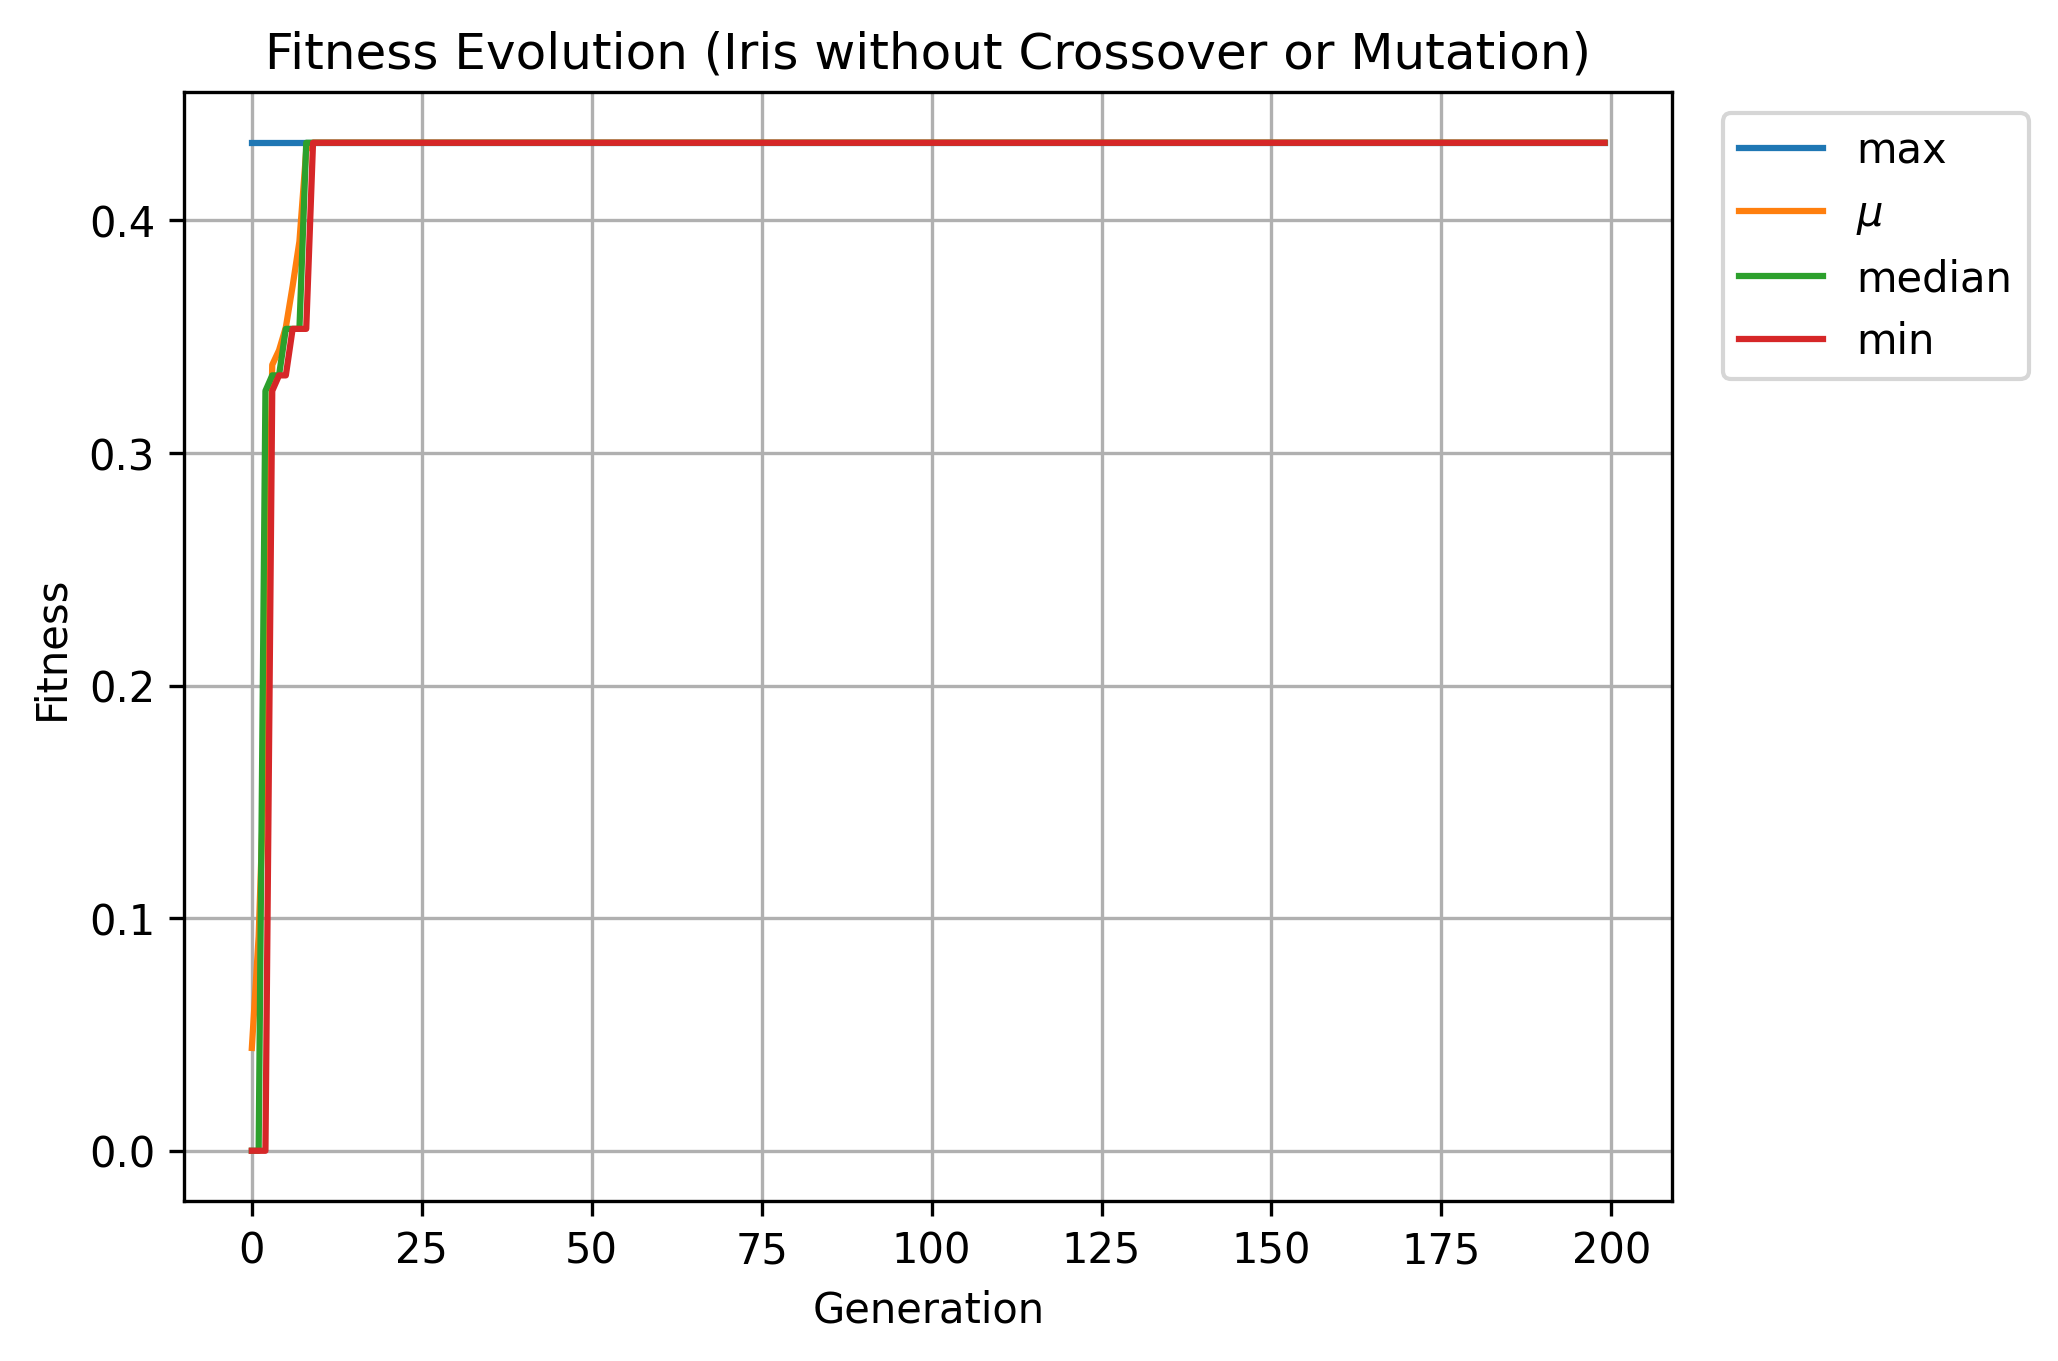
\includegraphics[width=\textwidth]{iris_baseline.png}
		\caption{LGP Without Variation On Iris}
		\label{fig:iris_baseline}
	\end{subfigure}
	\hfill
	\begin{subfigure}[b]{0.48\textwidth}
		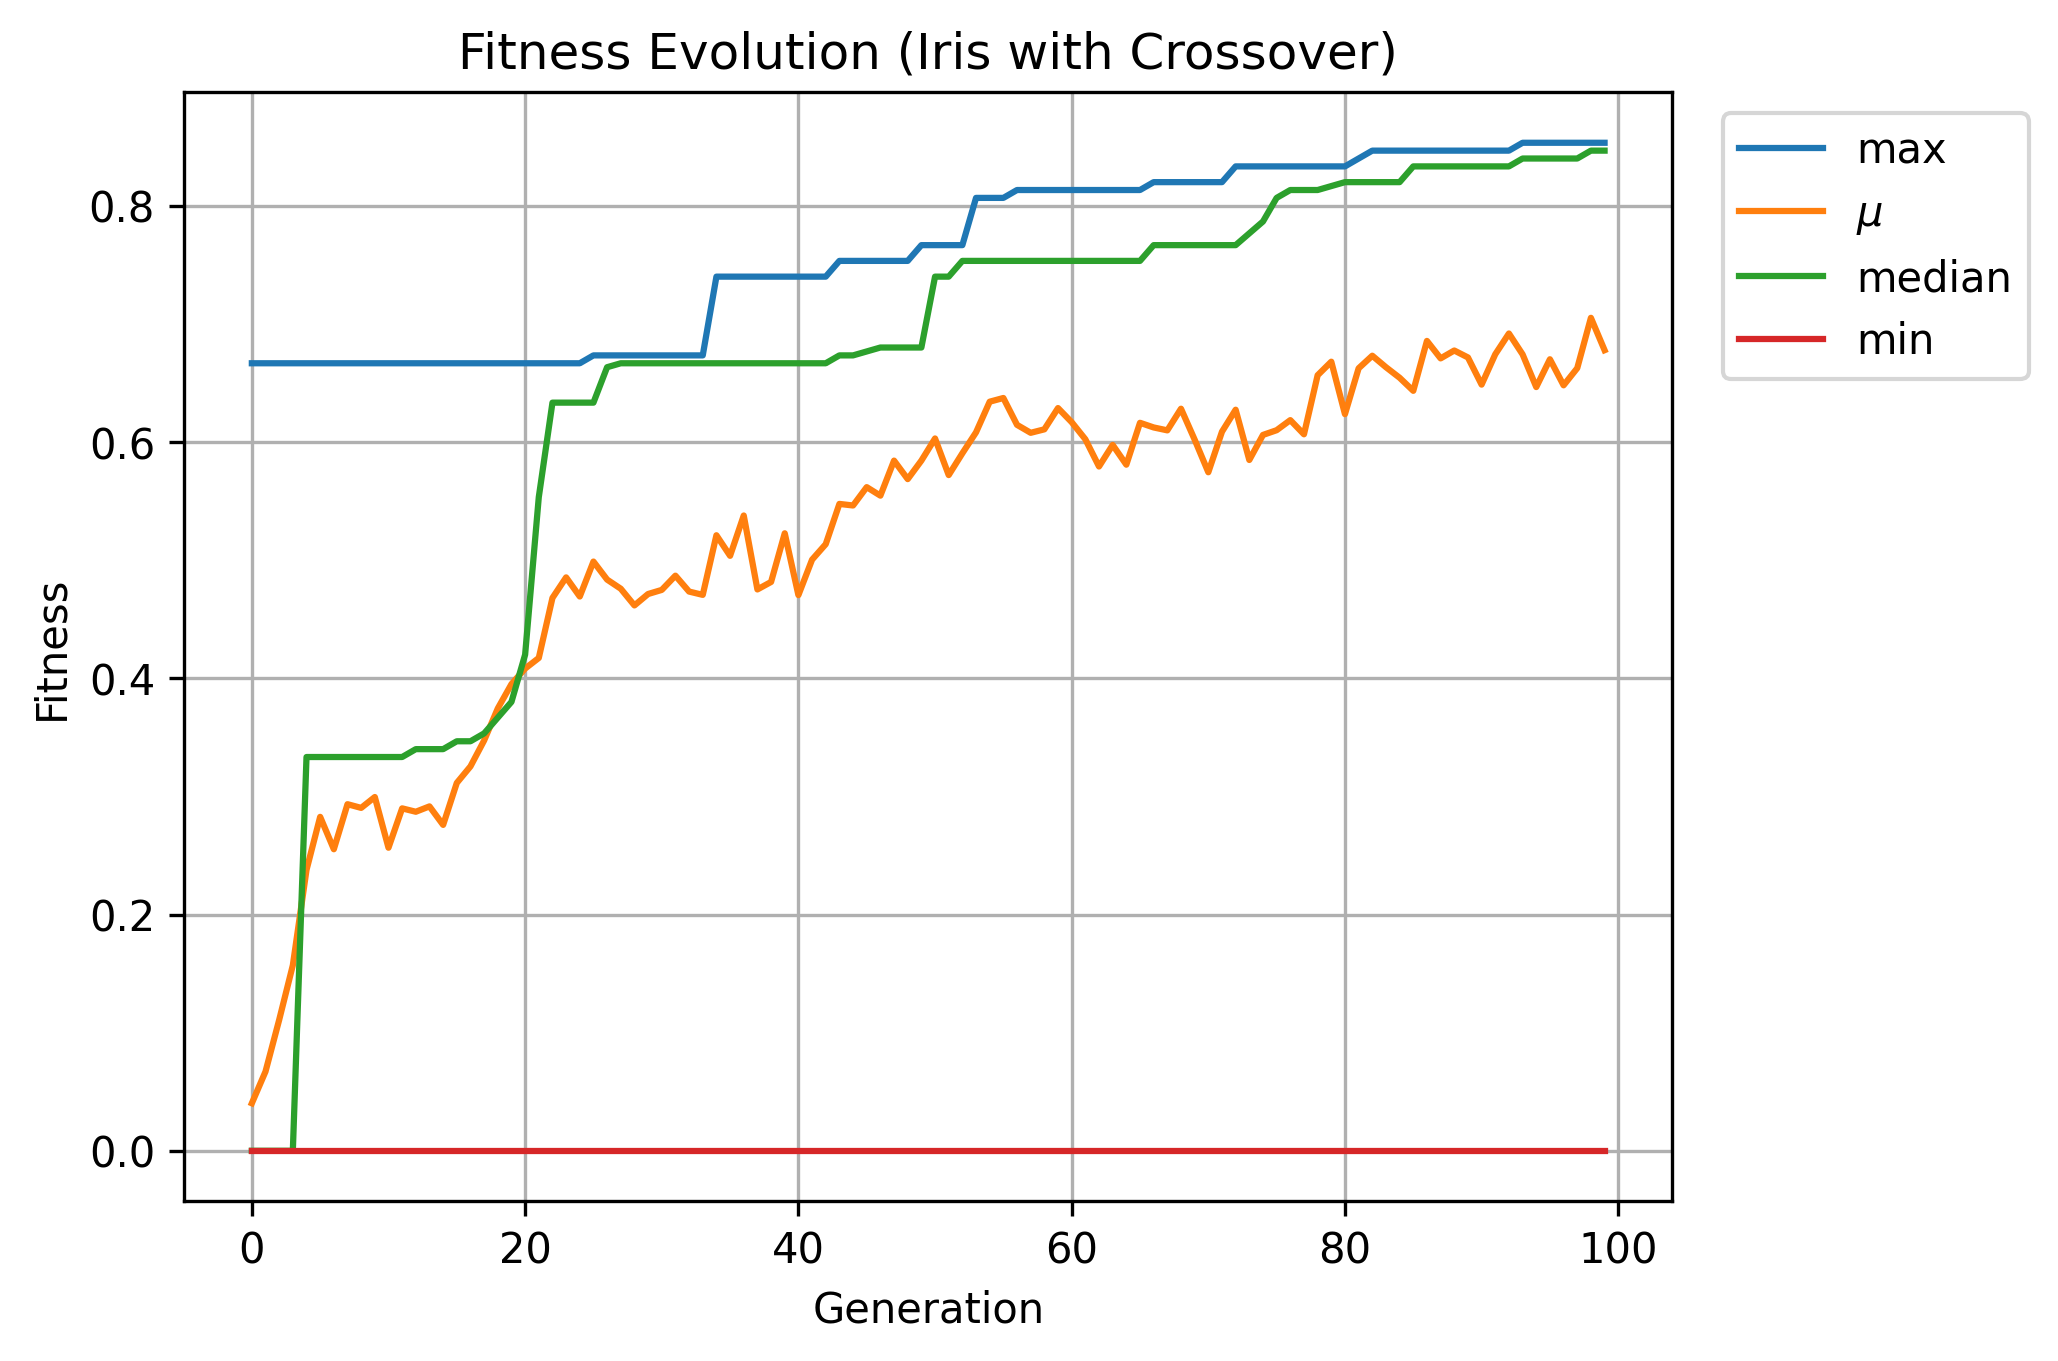
\includegraphics[width=\textwidth]{iris_crossover.png}
		\caption{LGP With Breed On Iris}
		\label{fig:iris_crossover}
	\end{subfigure}

	\medskip

	\begin{subfigure}[b]{0.48\textwidth}
		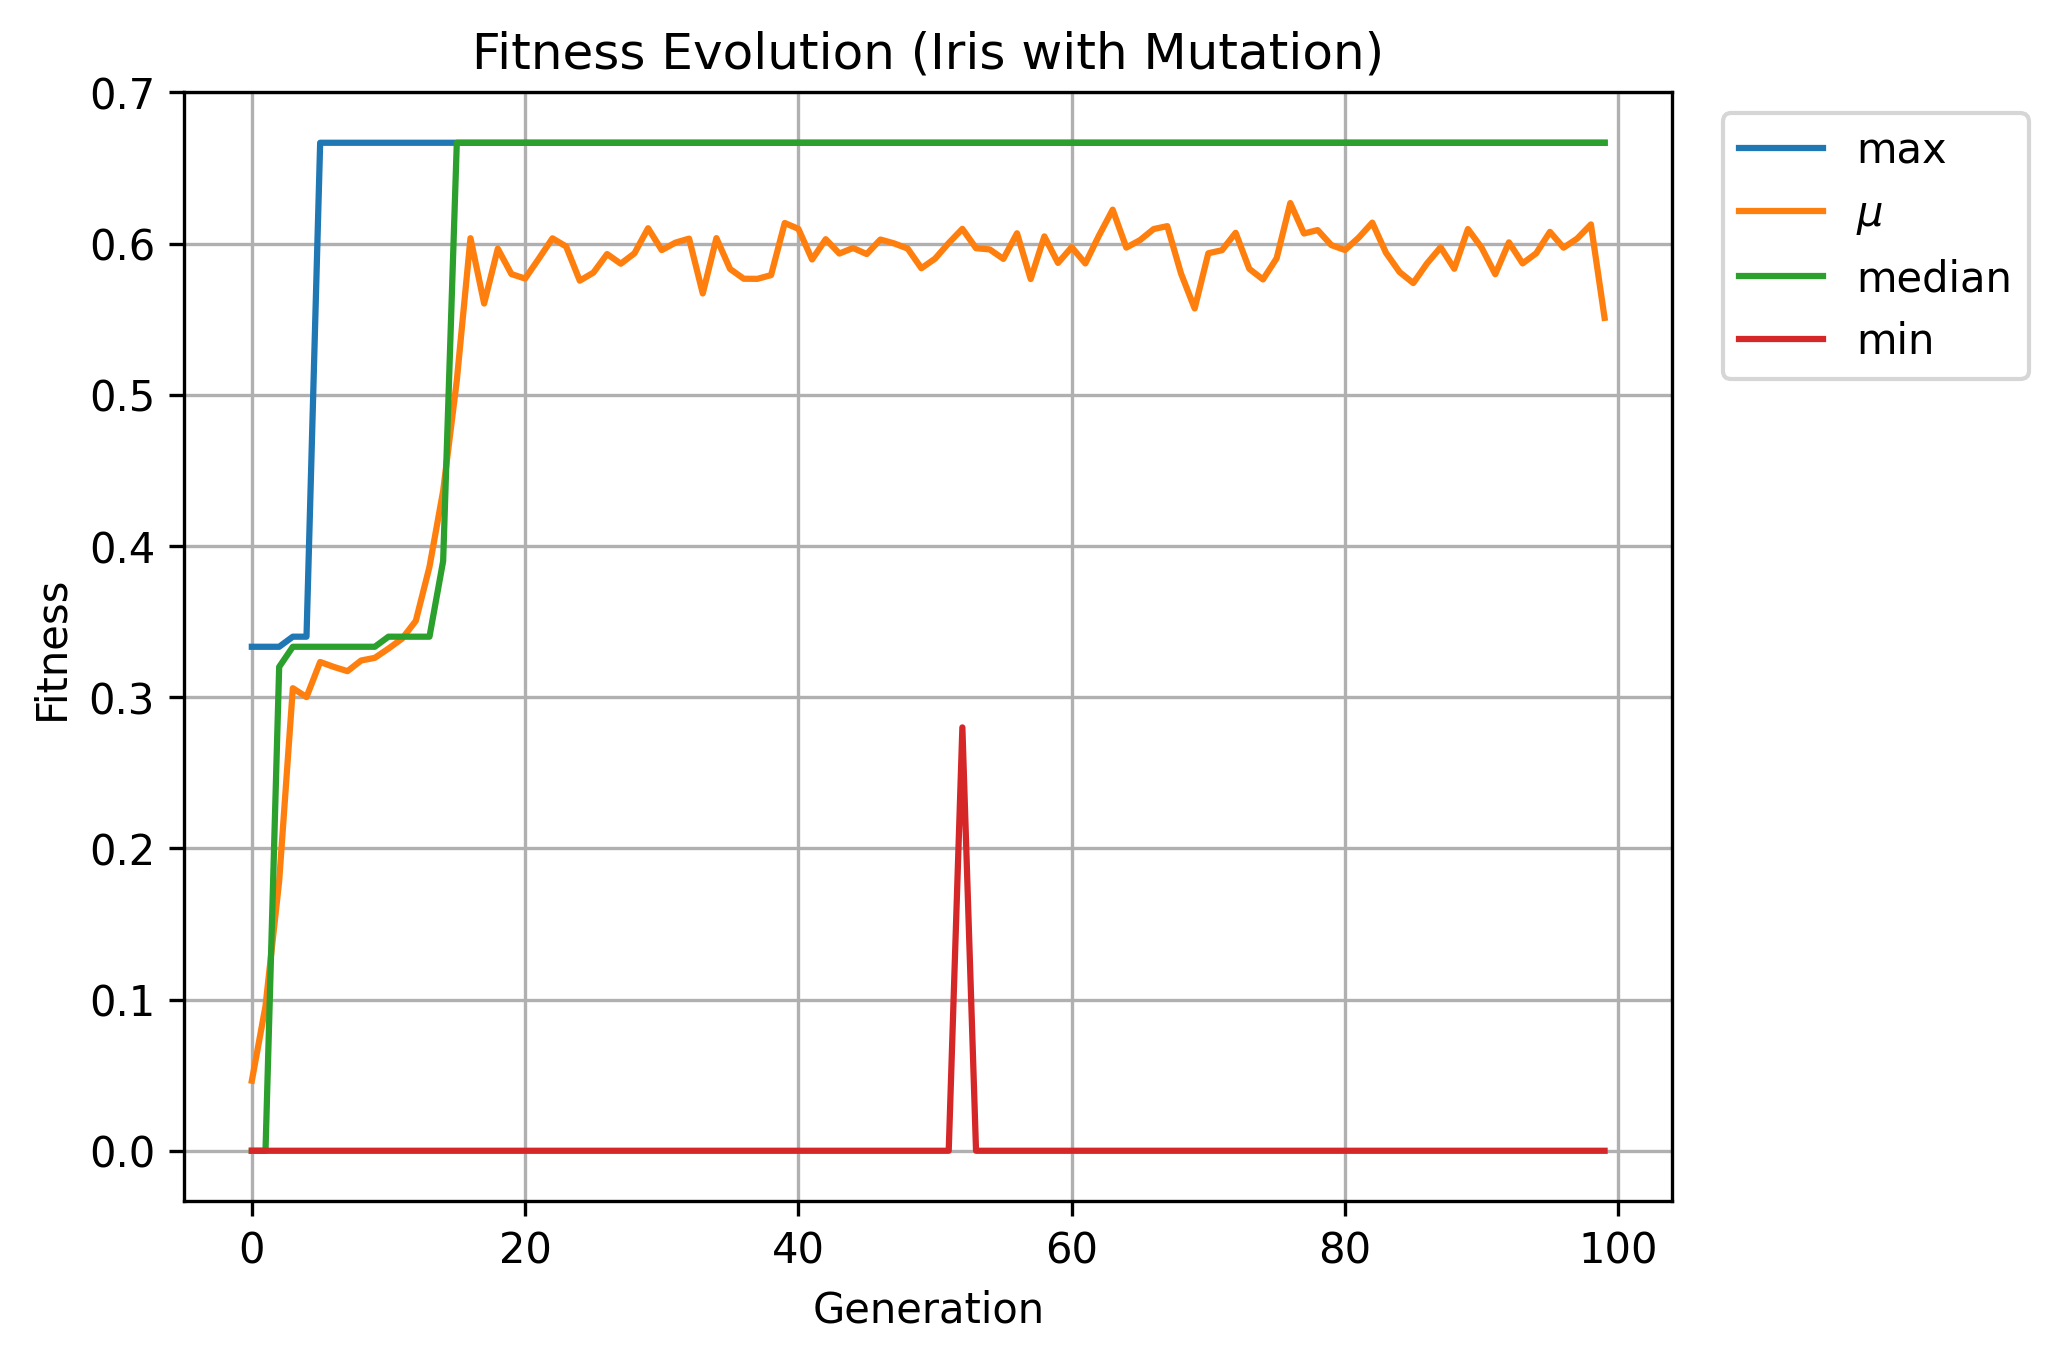
\includegraphics[width=\textwidth]{iris_mutation.png}
		\caption{LGP Using Only Mutation On Iris}
		\label{fig:iris_mutation}
	\end{subfigure}
	\hfill
	\begin{subfigure}[b]{0.48\textwidth}
		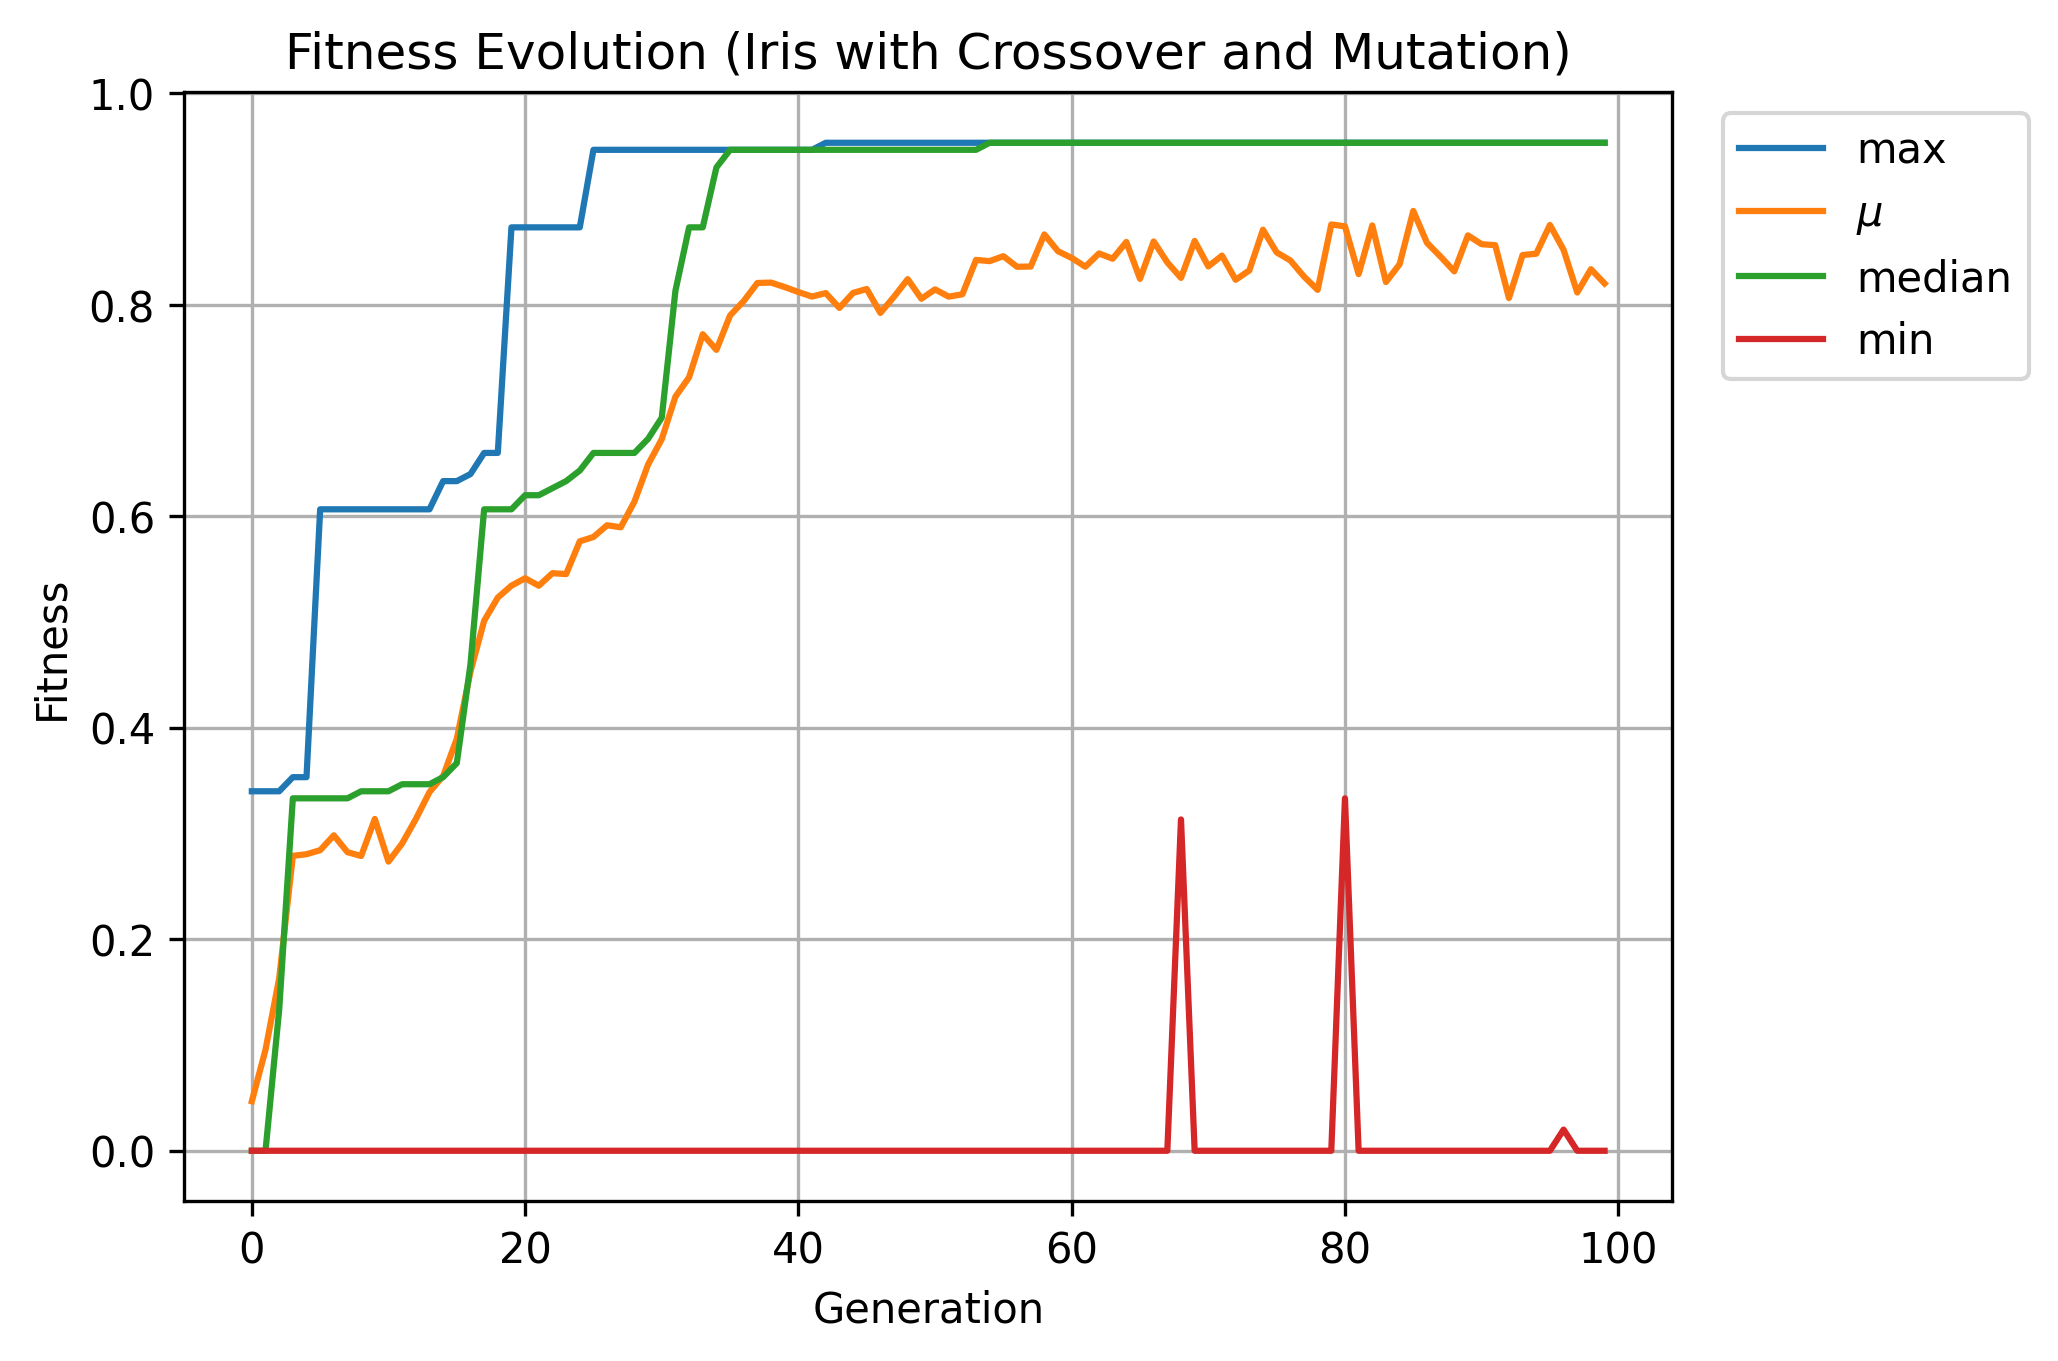
\includegraphics[width=\textwidth]{iris_full.png}
		\caption{LGP Using Both Mutation and Breeding On Iris}
		\label{fig:iris_full}
	\end{subfigure}

	\caption{Performance comparison of different genetic programming methods on iris dataset}
	\label{fig:iris_comparison}
\end{figure}

\section{Reinforcement Learning Integration}
We extend the fitness algorithm to work with both a Rust port of the OpenAI mountain car environment (mountain-car-v0) \cite{1606.01540} and the OpenAI cartpole environment (cartpole-v1) \cite{1606.01540}.

For the mountain-car-v0 environment, the agent's goal is to drive a car up a steep hill. The car is subject to gravity and has limited power. The car must learn to rock back and forth to build momentum before reaching the goal area at the top of the hill. The environment has two state variables representing the position, and velocity of the car. The car has three possible actions: push left, push right, or no push. The reward function for the environment gives a value of $-1$ at each time step until the car reaches the goal area, at which point the reward becomes $0$. The problem is considered solved when the car reaches the goal area with an average reward of -110 over 100 consecutive trials.

For the cartpole-v1 environment, the agent's goal is to balance a pole on top of a cart that can move left or right. The pole is subject to gravity, and the goal is to keep the pole upright for as long as possible. The environment has four continuous state variables representing the position and velocity of the cart and pole. The cart has two possible actions: move left or move right. The reward function for the environment gives a value of $1$ at each time step that the pole remains upright. The problem is considered solved when the pole remains upright for at least $195$ consecutive time steps over 100 consecutive trials.

With this in mind, we outline an alternative fitness algorithm used to baseline the framework on classical reinforcement learning problems, Algorithm \ref{alg:fitness-rl}.

\begin{algorithm}[hb]
	\caption{Fitness}
	\label{alg:fitness-rl}
	\begin{algorithmic}[1]
		\Procedure{Fitness}{$P, env$}
		\Comment{Given a program and an environment}
		\State{$score \gets 0$}
		\For{$i \in N_EPISODES$}
		\State{$done \gets False$}
		\While{$done = False$}
		\State{$output \gets \Call{Execute}{P, observation}$}
		\Comment{Execute the program for each input}
		\State{$action \gets \Call{Argmax}{output.action\_registers}$}
		\Comment{Argmax over the action registers}
		\State{$observation, reward, done, info \gets env.step(action)$}
		\Comment{Step the environment}
		\State{$score \gets score + reward$}
		\EndWhile
		\EndFor
		\State \textbf{return} $score$
		\EndProcedure
	\end{algorithmic}
\end{algorithm}


\section{Q Learning Integration}
We extend Algorithm \ref{alg:fitness-rl} further to support Q Learning (Algorithm \ref{alg:fitness-rlq}).
The Q Table consists of a 2D array of size $N_R \times N_A$, where $N_R$ is the number of registers the program can work with and $N_A$ is the number of available actions an agent can take. The Q Table is initialized to all zeros and updates only a different register has been selected. The Q Table is updated using the following formula.
\begin{equation}
	Q(R[x_t], a_t) \leftarrow Q(R[x_t], a_t) + \alpha \left(r_{t+1} + \gamma \max_a Q(R[x_{t+1}], a) - Q(R[x_t], a_t)\right)
\end{equation}

In this formula, $Q$ represents the Q Table, $R$ represents the set of registers, $a$ represents the available actions, $r_{t+1}$ is the reward at time step $t+1$, $\alpha$ is the learning rate, and $\gamma$ is the discount factor. The value $x_t$ represents the current state, while $x_{t+1}$ represents the next state. The update rule calculates the new Q value for the current state-action pair based on the observed reward and the maximum Q value for the next state.

\begin{algorithm}[hb]
	\caption{Q Learning LGP Fitness}
	\label{alg:fitness-rlq}
	\begin{algorithmic}[1]
		\Function{EvalFitness}{$P, S$}
		\State $sc \gets 0$
		\State $cur\_as \gets \Call{GetActionState}{S, P}$
		\If{$cur\_as = \text{None}$}
		\State \Return $-\infty$
		\EndIf
		\While{$st \gets \Call{S.Get}{} \neq \text{None}$}
		\State $rw \gets \Call{st.ExecuteAction}{cur\_as.action}$
		\State $sc \gets sc + rw$
		\If{$\Call{st.IsTerminal}{}$}
		\State \textbf{break}
		\EndIf
		\State $next\_as \gets \Call{GetActionState}{st, P}$
		\If{$next\_as = \text{None}$}
		\State \Return $-\infty$
		\EndIf
		\If{$cur\_as.register \neq next\_as.register$}
		\State $\Call{P.q\_table.Update}{cur\_as, rw, next\_as}$
		\EndIf
		\State $cur\_as \gets next\_as$
		\EndWhile
		\State \Return $sc$
		\EndFunction
	\end{algorithmic}
\end{algorithm}

\section{Experimental Setup}

In this section, we outline the experimental setup used to evaluate the performance of the proposed Q-Learning LGP algorithm in comparison to the baseline LGP. The experiments were conducted in two main stages: hyperparameter optimization and performance evaluation.

\subsection{Hyperparameter Optimization}

First, we utilized the Optuna hyperparameter optimization library \cite{akiba2019optuna} to find the optimal parameters for the baseline LGP programs. Optuna is a flexible and efficient hyperparameter optimization framework that allows for the automatic exploration of hyperparameter spaces in search of the best settings for a given algorithm.

Once the optimal parameters for the baseline LGP programs were identified, we conducted a separate search using Optuna to find the optimal Q-Learning constants for the Reinforced Linear Genetic Programming (RLGP) programs. This process aimed to fine-tune the RLGP algorithm's performance by selecting the most suitable Q-Learning parameters based on the problem domain and the characteristics of the LGP framework.

\subsection{Performance Evaluation}

After obtaining the optimal parameters for both baseline LGP and RLGP, we proceeded with the performance evaluation phase. This stage involved conducting 100 experiments, each consisting of 100 trials. The goal of these experiments was to assess the effectiveness and robustness of the RLGP algorithm compared to the baseline LGP across multiple runs and problem instances.

For each experiment, we calculated the mean, median, minimum, and maximum performance scores obtained by both baseline LGP and RLGP. These summary statistics provided a comprehensive overview of the algorithms' performance, highlighting their strengths and weaknesses across different trials and problem instances.

Finally, we plotted the average results (mean, median, min, max) for each experiment to visually compare the performance of the baseline LGP and RLGP algorithms. This visualization allowed us to identify trends and patterns in the algorithms' performance and gain insights into the benefits of incorporating Q-Learning into the LGP framework.

By following this experimental setup, we aimed to provide a thorough and unbiased evaluation of the proposed Q-Learning LGP algorithm, demonstrating its potential advantages over the baseline LGP and paving the way for future research and development in this area.

\chapter{Analysis}

This chapter analyzes the performance of a population of programs trained using Linear Genetic Programming (LGP)
and a population of programs trained using Linear Genetic Programming Reinforced with Q-Learning (LGP-Q). The programs
are trained on the cartpole-v1 and mountain-car-v0 environments \cite{1606.01540} as mentioned in the Reinforcment Integration section.
Once the results are explained, we analyze them to provide insight into the impact of Q-Learning on the performance of LGP. Note that we use the definition of done as referenced in the leaderboards, see \href{https://github.com/openai/gym/wiki/Leaderboard}{OpenAI Gym Leaderboard Wiki}.

\section{Experimental Results}

\subsection{Cart Pole}

Figure \ref{fig:cart-pole-comparison} shows a comparison of the two frameworks performance on the cartpole-v0 task. Over 100 exeriments, we observe that LGP averages a maxmium of 466, a median of 454, a median of 466 and minimum of 128. On the other hand, RLGP
averages a maximum of 213, a median of 207, a mean of 213 a minimum of 31. In both cases,the population of the respective frameworks were able solve the problem. Both frameworks were able
to generate a program in the first 10 generations that was able to solve the problem. However, the RLGP framework immediately plateaus, whilst the LGP framework continues to improve until hitting a plateau at 80 generations.

\begin{figure}[hb]
	\centering
	\begin{subfigure}{1.0\textwidth}
		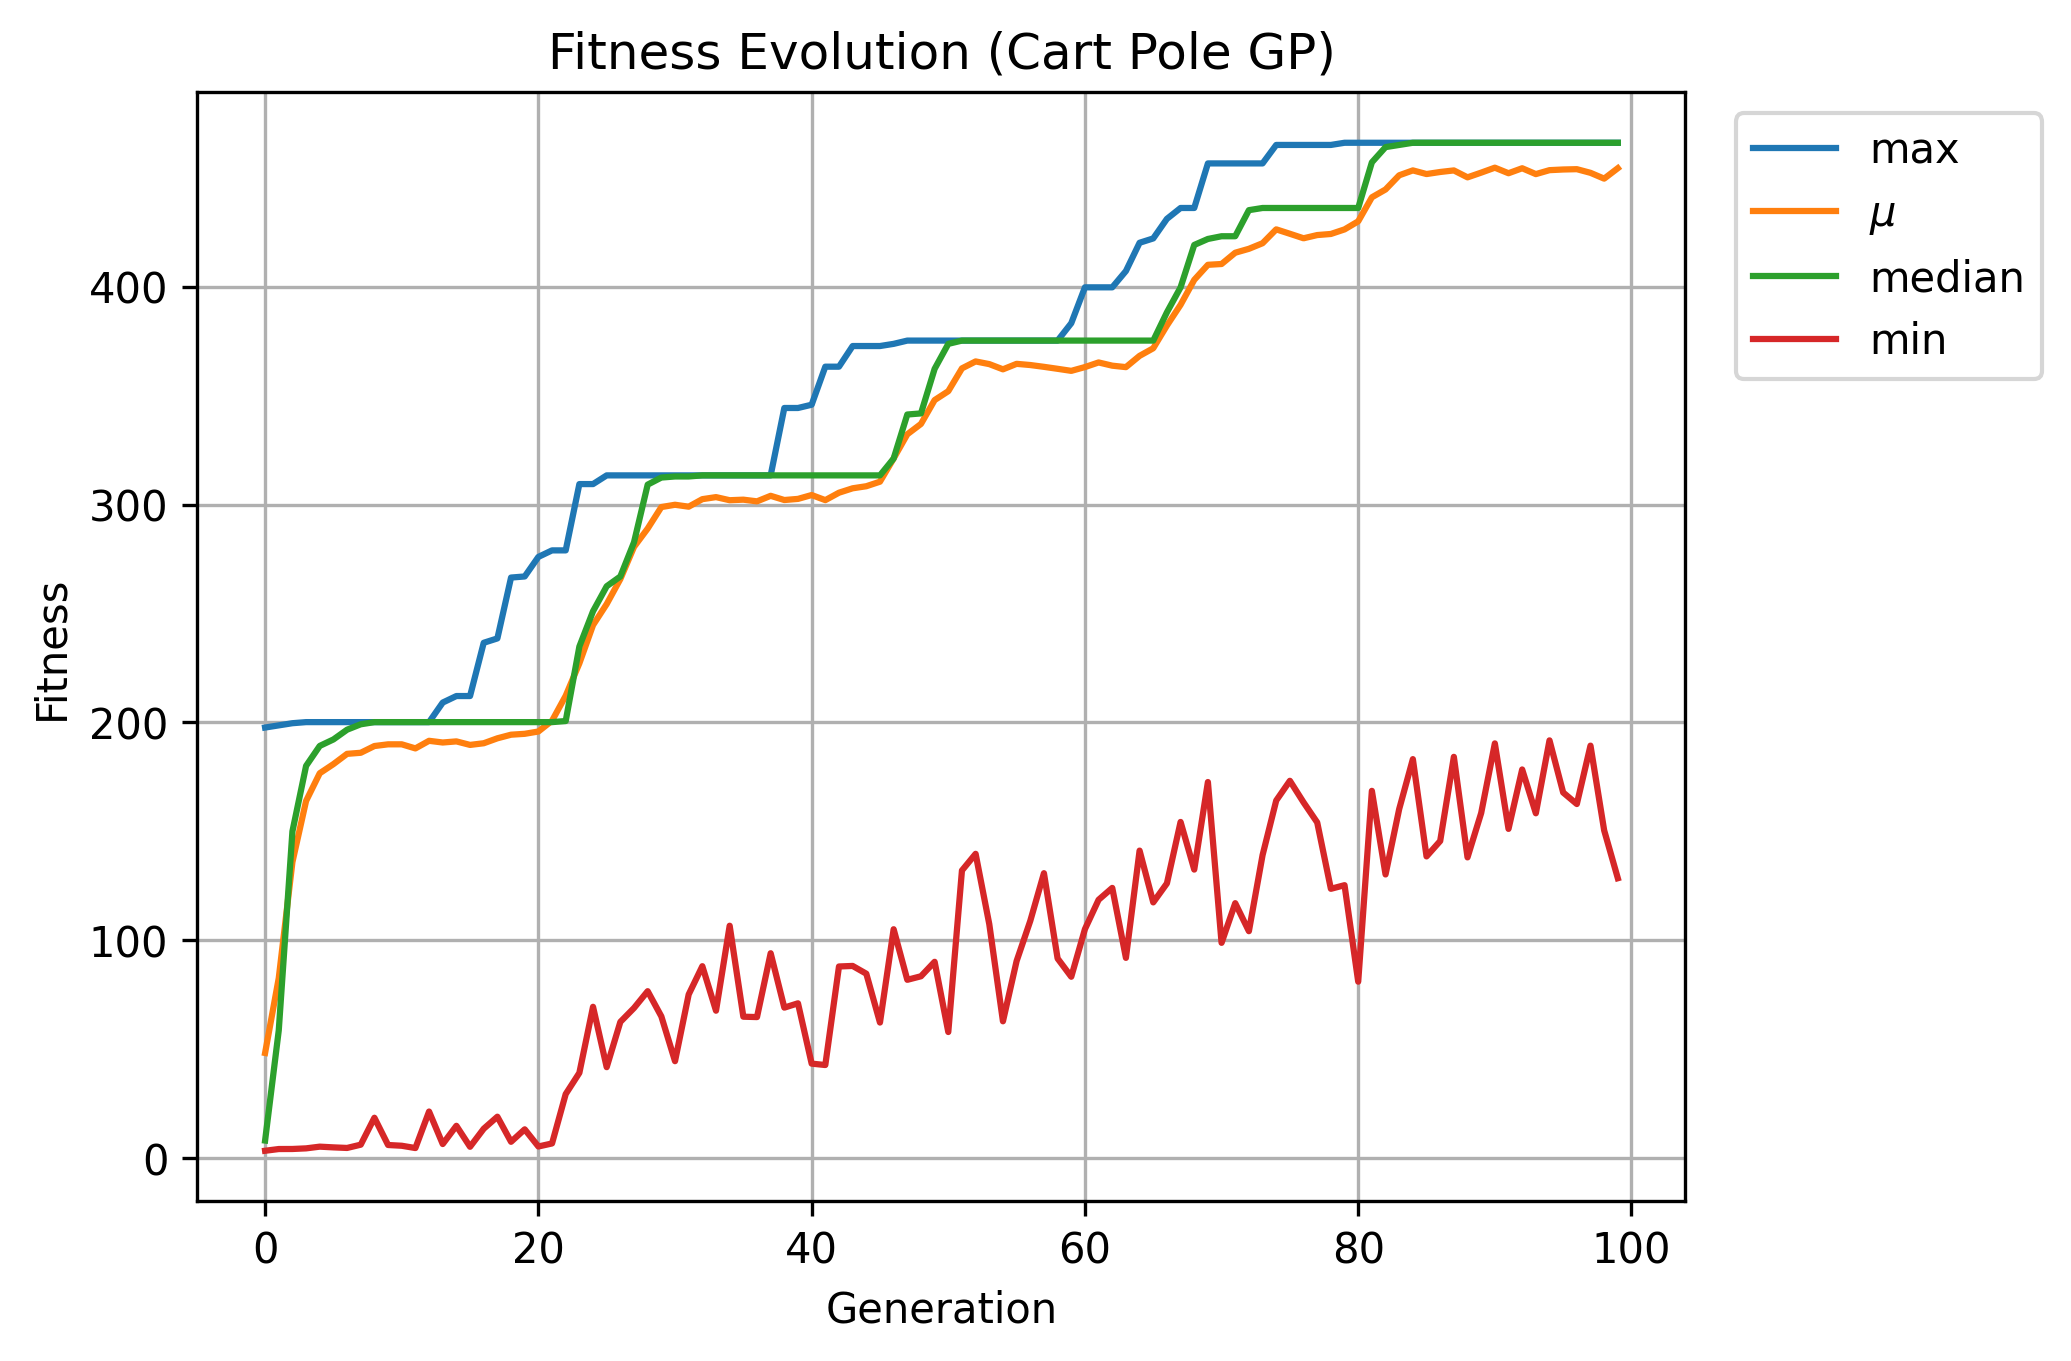
\includegraphics[width=\linewidth]{cart_pole_lgp.png}
		\caption{LGP cart-pole-v0}
		\label{fig:cart-pole-lgp}
	\end{subfigure}
	\hfill
	\begin{subfigure}{1.0\textwidth}
		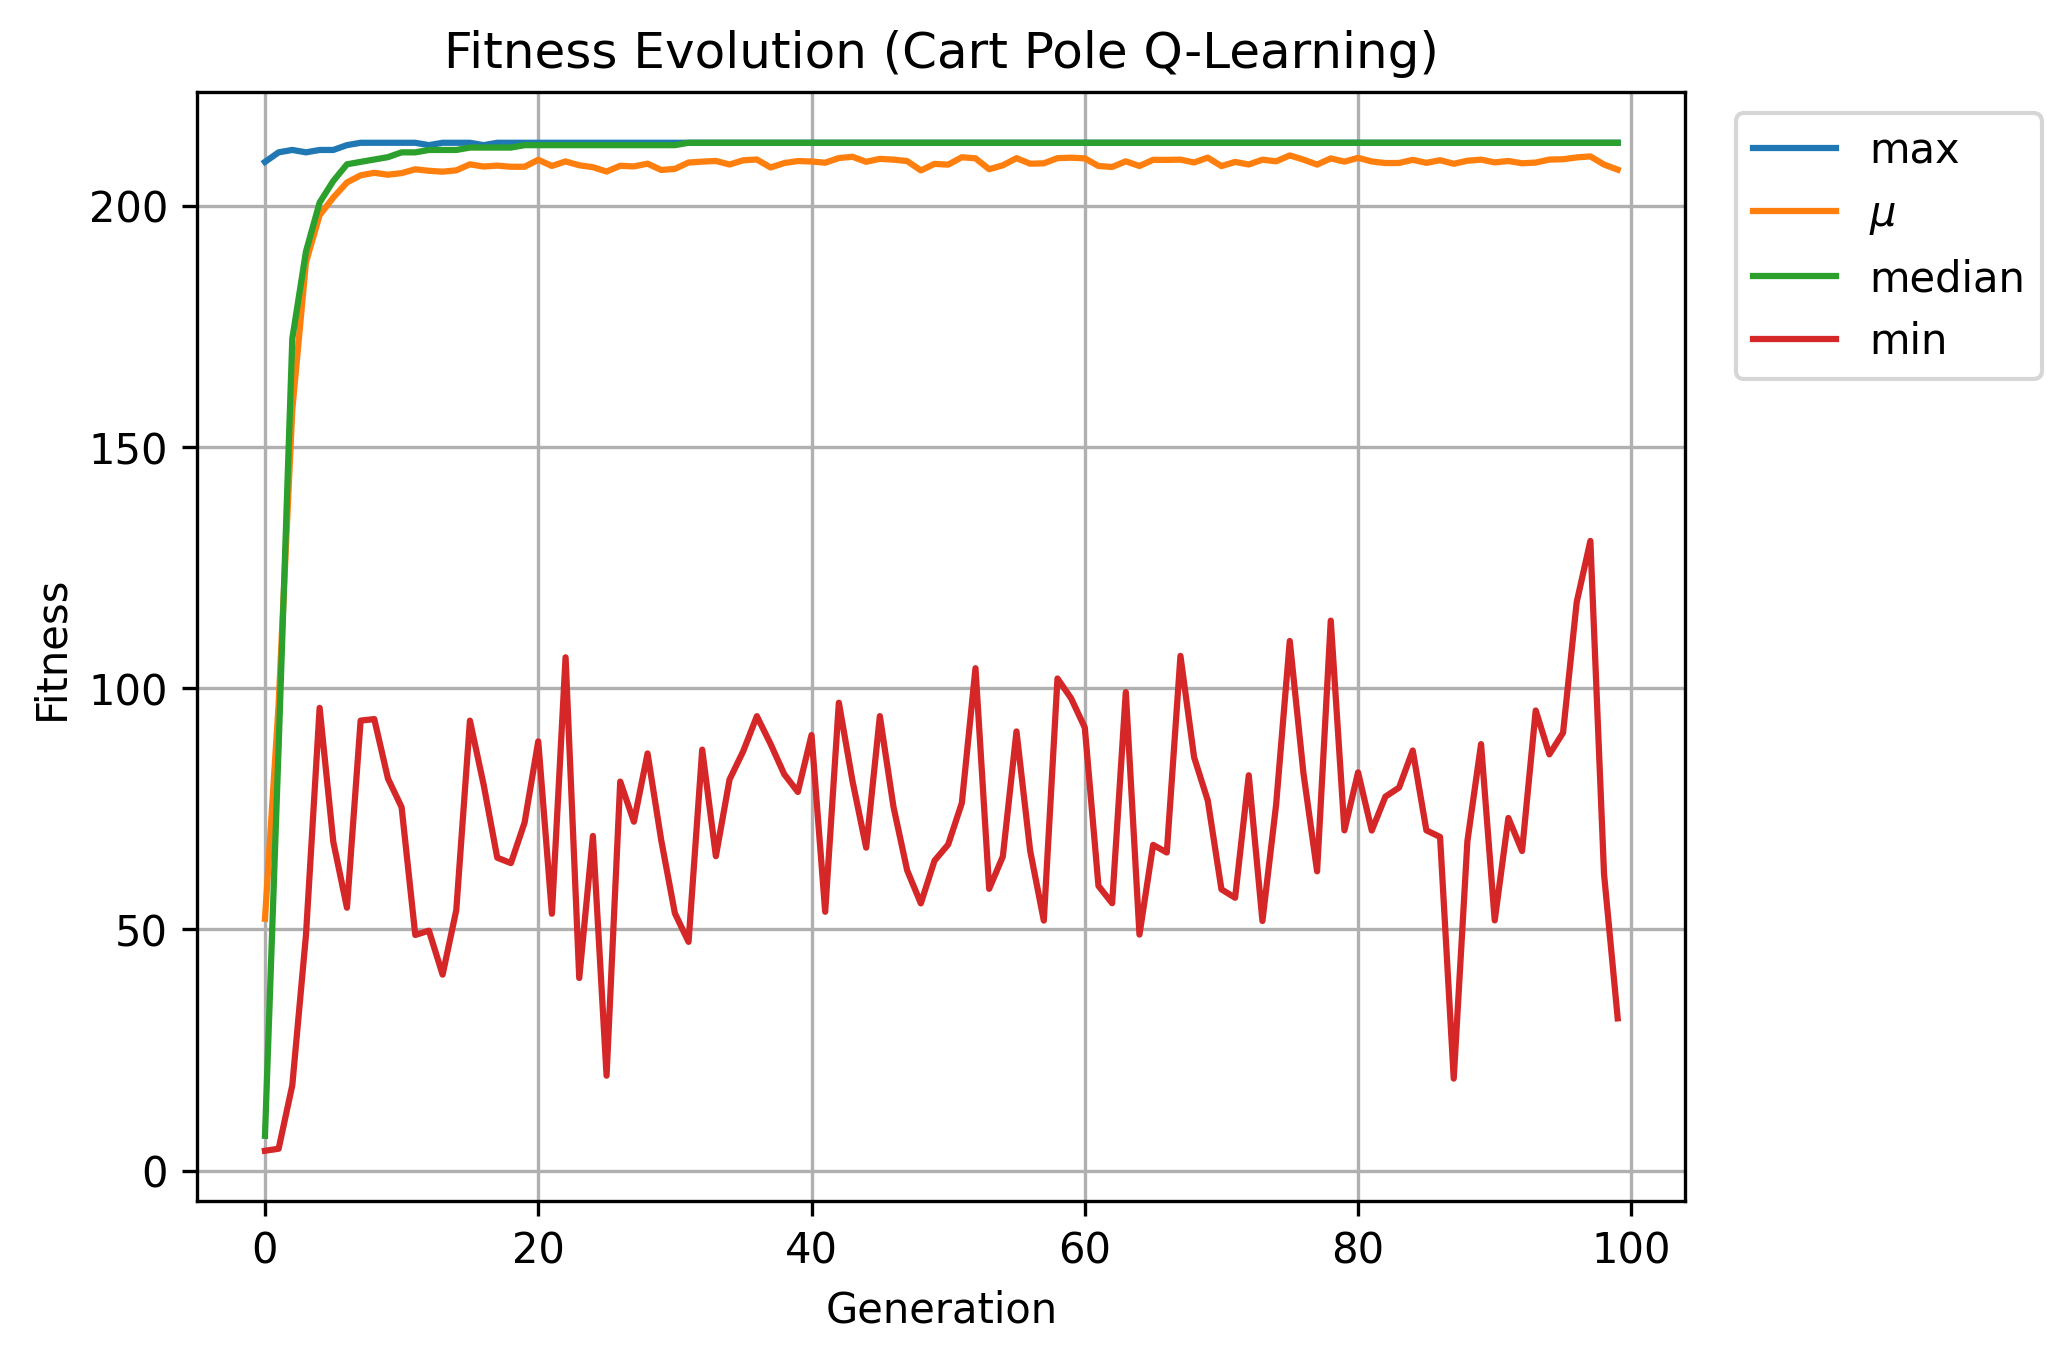
\includegraphics[width=\linewidth]{cart_pole_q.png}
		\caption{RLGP cart-pole-v0}
		\label{fig:cart-pole-q}
	\end{subfigure}
	\caption{Comparison of Cart Pole}
	\label{fig:cart-pole-comparison}
\end{figure}


\subsection{Mountain Car}

Figure \ref{fig:mountain-car-comparison} demonstrates a similar pattern to that of the cartpole-v0 task. The RLGP framework falls short of solving the task, averaging a max of -114, a mean of-130, a median of -117.6685 and a min of -200. On the other hand, the LGP framework is able to solve the task, albeit narrowly, averaging a max -106, a mean of -126, a median of -120,and a min -200.0. Here, we observe that RLGP achieves a higher median score, with a slight upward trend whereas the LGP achieves a lower median, with no particular trend in any direction. Both of these framework look as they quickly converge to a value and then plateau.

\begin{figure}[ht]
	\centering
	\begin{subfigure}{1.0\textwidth}
		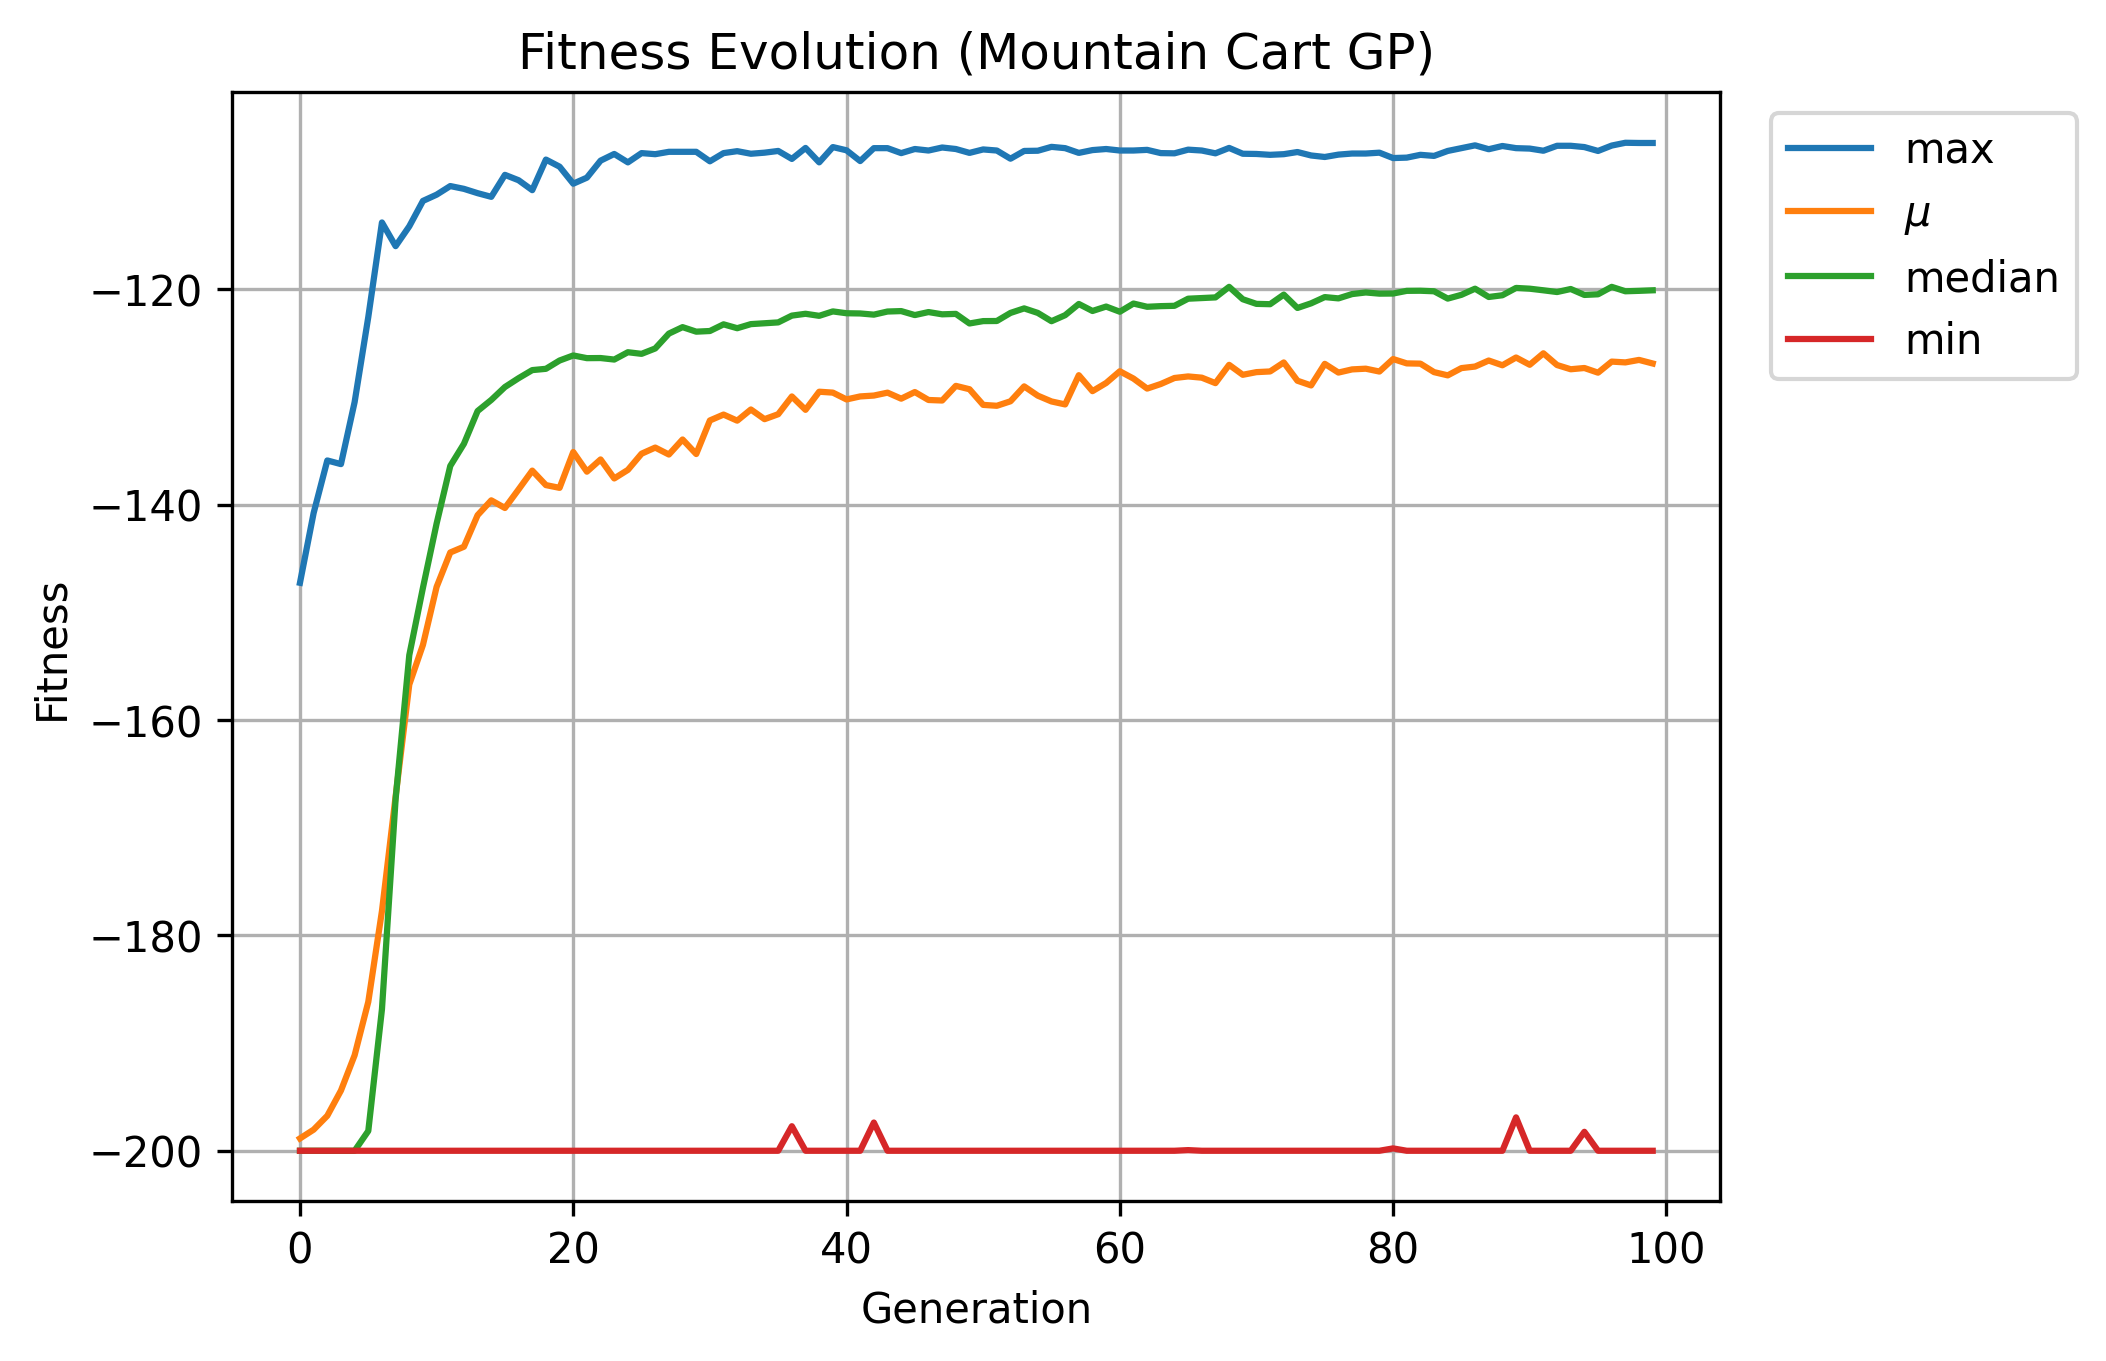
\includegraphics[width=\linewidth]{mountain_car_lgp.png}
		\caption{Baseline Linear Genetic Programming}
		\label{fig:mountain-car-lgp}
	\end{subfigure}
	\hfill
	\begin{subfigure}{1.0\textwidth}
		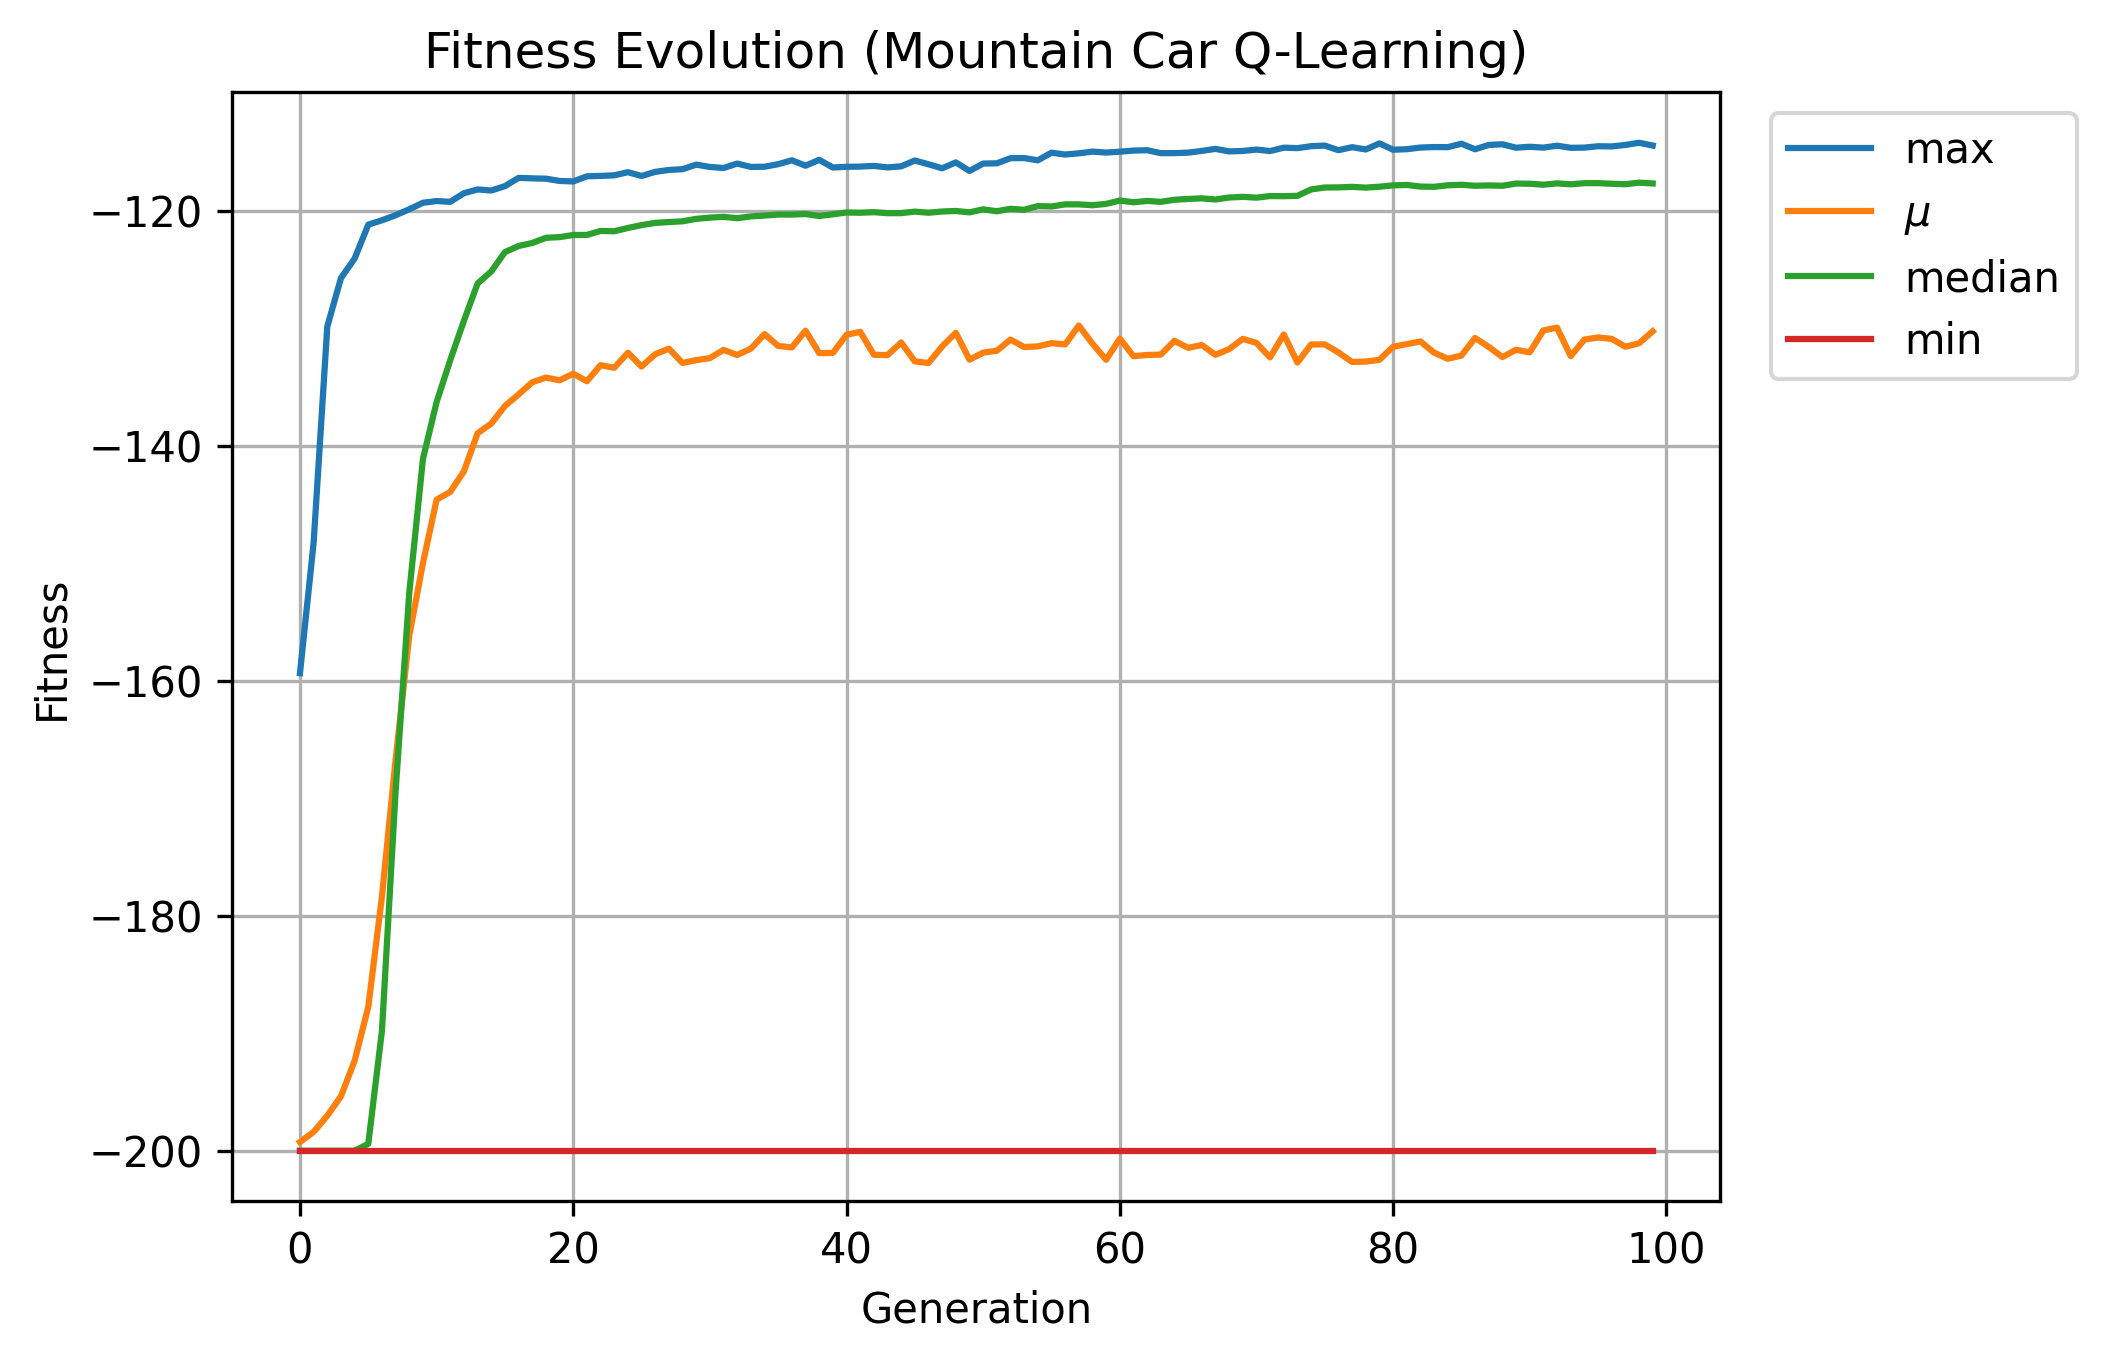
\includegraphics[width=\linewidth]{mountain_car_q.png}
		\caption{Linear Genetic Programming Reinforced with Q-Learning}
		\label{fig:mountain-car-q}
	\end{subfigure}
	\caption{Comparison of Mountain Car}
	\label{fig:mountain-car-comparison}
\end{figure}

\section{Discussion}

Initially, we would have expected for the frameworks to perform better on mountain-car-v0 than cart-pole-v1 as the state space is much simpler (one consists of 2 state properties whilst the other contains four). However, the opposite seems to be true,
the cart pole task was able to be solved relatively easily in comparison to the mountain car task, in which RLGP failed to solve the problem. One explaination for this discrepancy is the difference in the nature of the tasks. The cart-pole task is inherently more continuous, allowing for small adjustments to have a direct impact on the balancing of the pole. On the other hand, the mountain car task requires more strategic and discrete actions to build up momentum and reach the goal. This may indicate that the LGP and RLGP frameworks are better suited to tackle continuous control problems.

Another contributing factor could be the exploration-exploitation trade-off present in RLGP. The Q-learning component might not be exploring the state space effectively, thus getting stuck in local optima and hindering the overall performance. In contrast, the LGP framework seems to be more robust in its exploration of the solution space, enabling it to perform better on both tasks.

Moreover, the difference in performance may also be attributed to the limitations of the genetic programming approach. While LGP and RLGP are capable of discovering compact and interpretable representations of policies, they are not guaranteed to find the global optimum. The search process depends on the initial population and variation operators, which can impact the quality of the solutions found. The experimental set up might have been poor, and the parameters beneifical to LGP might not have been optimal for RLGP. Its possible that
we could've seen better results if Q leanring parameters was not simply a wrapper on top of a preexisting configuration.

In conclusion, our experiments demonstrate that the LGP framework outperforms the RLGP framework in both cart-pole and mountain car tasks. Although both frameworks were able to solve the cart-pole task, RLGP failed to solve the mountain car task, suggesting that the integration of Q-learning into genetic programming may not always lead to improved performance. Future work could involve investigating alternative reinforcement learning algorithms, adapting exploration strategies, or incorporating domain knowledge to enhance the performance of genetic programming-based frameworks. Additionally, it would be valuable to test these frameworks on a broader range of tasks to better understand their strengths and limitations.

\chapter{Conclusion}

Due to the amount of time spent on reconfiguring the framework in addition to the short nature of this research project,
various forms of experimentation did not occur. With the further optimization of hyperparameters and a different experimental setup, its possible that results could have improved. Nonetheless, the framework now exists for experimenting with easy, and opens a door for further exploration into the subject at hand. In the future, we would like to
explore different benchmarking approaches and different types of tasks besides those found in the classical control module \cite{1606.01540}, as it might bring forth insight about the types of problems where RLGP can thrive.

\bibliographystyle{plain}
\bibliography{thesis}

\end{document}
